%BAB_2 LAPORAN KP
\chapter{LANDASAN TEORI}

\section{SCARA Robot}
	\textit{Selective Compliance Articulated Robot Arm} atau SCARA merupakan robot yang memiliki empat \textit{deggres of freedom} (DOF). Robot jenis ini memiliki dua atau tiga \textit{horizontal joint} yaitu bagian \textit{shoulder,elbow}dan\textit{wrist} yang dikendalikan oleh servo, sedangkan pada bagian \textit{vertical joint} dikendalikan dengan pneumatik. Sehingga, gerakan yang terdapat pada robot SCARA dapat diklasifikasikan sebagai gerakan mengambil dan menempatkan object. penelitian ini menggunakan robot SCARA dengan nama Serpent-1. Serpent-1 memiliki tiga buah motor servo untuk mengatur pergerakan pada bagian \textit{shoulder,elbow},dan\textit{wrist}. sedangkan pada \textit{vertical joint} dan gerakan capit menggunakan mekanisme pneumatik.spesifikasi fisik dari robot Serpent-1 dapat dilihat pada tabel 2.1 berikut.

\begin{table}[H]
	\centering
	\caption{Spesifikasi Robot SCARA}
	\resizebox{6cm}{!}{%
		\begin{tabular}{|l|l|}
			\hline
			Main arm length      & $$\hspace{2cm} 		\\ \hline
			Fore arm length      & $$  				\\ \hline
			Shoulder movement    & $$\textdegree   		\\ \hline
			Elbow movement       & $$\textdegree   		\\ \hline
			Wrist rotation       & $$\textdegree 		\\ \hline
			Up \& down movement  & $$   				\\ \hline
			Maximum tip velocity & $$  				\\ \hline
			Capacity             & $$  				\\ \hline
		\end{tabular}%
	}
\end{table}

\section{Motor servo}
	Motor servo merupakan sebuah motor DC yang memiliki sistem \textit{feedback}. \textit{feedback} pada motor servo merupakan koreksi sudut motor DC terhadap sudut referensi \cite{Younkin2002}. pada robot Serpent-1 terdapat tiga buah motor DC, motor DC	 bagian wrist dan elbow merupakan motor DC yang identik.sehingga penulis hanya fokus membandingkan spesifikasi dua motor DC yaitu motor DC yang berada di bagian shoulder (\textit{main arm}) dan motor DC yang berada di bagian elbow (\textit{fore arm}). spesifikasi dua motor DC tersebut dapat dilihat pada tabel 2.2 sebagai berikut

\begin{table}[H]
	\centering
	\caption{Spesifikasi Motor DC pada robot Serpent-1}
	\resizebox{11cm}{!}{%
		\begin{tabular}{|l|l|}
			\hline
			Moments of inertia of the main arm ($J_{1}$)    							& $0.0980kgm^{2}$ 				\\ \hline
			Moments of inertia of the fore arm ($J_{2}$)    							& $0.0115 kgm^{2}$ 				\\ \hline
			Masses of the main arm	($m_{1}$)											& $1.90kg$   					\\ \hline
			Masses of the fore arm  ($m_{2}$)     										& $0.93kg$   					\\ \hline
			Motor and equivalent inertias ($J_{m}$)      								& $3.3*10^{-6}kgm^{2}$ 			\\ \hline
			Back emf constants for main arm and fore arm motor ($K_{e1}=K_{e2}$)  		& $0.047Nm/A$   				\\ \hline
			Armature resistance for main arm and fore arm motor($R_{a1}=R_{a2}$)		& $3.5\Omega$  					\\ \hline
			Armatures inductances for main and fore arm motor  ($L_{a1}=L_{a2}$) 		& $1.3mH$ 						\\ \hline
		\end{tabular}%
	}
\end{table}

\section{Kinematika model \textit{elbow planar} Denavit-Hartenberg}
	Kinematika model \textit{elbow planar} Denavit-Hartenberg merupakan persamaan yang digunakan untuk mencari nilai sudut yang tepat pada bagian \textit{shoulder} dan \textit{elbow} dari input koordinat kartesius yang diberikan dengan tepat\cite{Spong2006}. gambar model \textit{elbow planar manipulator} dapat dilihat dari gambar berikut.
	\begin{figure}[H]
		\centering
		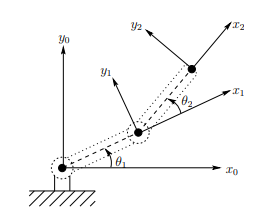
\includegraphics[width=6cm]{gambar/model.png}
		\caption{model \textit{elbow planar manipulator}}
	\end{figure}
	Persamaan kinematika dari gambar diatas dapat dirumuskan sebagai berikut :
	
	\begin{align}
	x_{2}&= a_{1}\cos\theta_{1}+a_{2}\cos(\theta_{1}+\theta_{2})\\
	y_{2}&= a_{1}\sin\theta_{1}+a_{2}\sin(\theta_{1}+\theta_{2})
	\end{align}
	
	persamaan 1 dan persamaan 2 dapat disusun ulang menjadi \textit{invers kinematic} dengan cara menempatkan sudut dari shoulder dan elbow ($\theta_{1}$,$\theta_{2}$) menjadi output dari persamaan tersebut. sedangkan input persamaan model tersebut adalah koordinat sumbu $x_{1}$ dan $x_{2}$.Sehingga,persamaan tersebut menjadi berikut :
	
	\begin{align}
	\cos\theta_{2}&=\frac{(x^{2}_{\mathrm{2}}+y^{2}_{\mathrm{2}})-(a^{2}_{\mathrm{1}}+a^{2}_{\mathrm{1}})}{2a_{1}a_{2}}\\
	\nonumber
	&\\
	\tan\theta_{1}&=\frac{-(a_{2}\sin\theta_{2})x_{2}+(a_{1}+a_{2}\cos\theta_{2})y_{2}}{(a_{2}\sin\theta_{2})y_{2}+(a_{1}+a_{2}\cos\theta_{2})x_{2}}
	\end{align}
	
\section{LabVIEW}
	LabVIEW adalah sebuah \textit{ghrapical programming language} yang dikembangkan oleh National instrumens. Program pada LabVIEW terdiri atas dua jendela program yang aktif, yaitu \textit{front panel} dan \textit{block diagram}. Panel \textit{block diagram} merupakan tempat user untuk menuliskan program. bagian \textit{front panel} adalah tempat mengatur tampilan antar muka dari LabVIEW serta tempat untuk menambahkan berbagai jenis \textit{switch,knob,slider,graph} dan lain-lain. Dalam penelitian ini LabVIEW berfungsi sebagai antar muka antara user dengan hardware Serpent-1. Antar muka ini mengirimkan data berupa posisi titik koordinat $x_{2}$ dan $x_{2}$ kepada mikrokontroller Arduino Mega 2560 dan mengamati feedback dari sensor encoder pada robot Serpent-1 berupa sudut elbow dan sudut shoulder.
\section{\textit{Microcontroller}}
	Arduino Mega 2560 merupakan \textit{microcontroller} dengan chip ATMega 2560. \textit{Microcontroller} ini memiliki 54 pin \textit{digital input} yang juga dapat difungsikan sebagai pin \textit{digital output}, terdapat 15 pin yang digunakan sebagai PWM \textit{output}, 16 pin input analog, empat UARTs (\textit{hardware serial ports}),16MHz \textit{crystal oscillator},sebuah konektor USB,\textit{power jack},ICSP \textit{header}, dan sebuah \textit{reset button}.Pada penelitian ini, Arduino Mega 2560 digunakan sebagai kontroller pada robot Serpent-1.
	
	\begin{figure}[H]
		\centering
		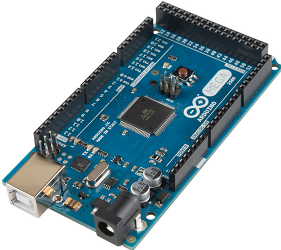
\includegraphics[width=4.33cm]{gambar/arduino_mega.png}
		\caption{\textit{Microcontroller} Arduino Mega 2560}
	\end{figure}